%issue with tkz-berge.sty and tkz-graph being removed from 2020 release of texlive:
% https://tex.stackexchange.com/questions/547173/texlive-2020-how-to-deal-with-tikz-berge-and-tikz-kiviat-packages-that-were-rem
% just downloaded the .sty files and added them to local folder i'm compiling this doc in! 

%https://www.youtube.com/watch?v=Lli99OmkPwM

%i guess if they get to drop a Pset, I don't want each to count as 9 points...want a number divisible by 8 lol; or I could do each is worth 10 points and give them a freebie? or play with the participation some more! 

\documentclass[11pt, a4paper]{article}
\usepackage[inner=2cm,outer=2cm,top=3cm,bottom=3cm]{geometry}
\pagestyle{empty}
\usepackage{graphicx}
\usepackage{tikz}
\usepackage{pgfplots}
\usepackage{bm}
\usepackage{multicol}
\usepackage{amssymb}
\usepackage{amsmath}

%\usetikzlibrary{snakes}
%\usetikzlibrary{lindenmayersystems}
\usetikzlibrary{arrows,petri,topaths}
\usetikzlibrary{plotmarks}
\usepackage{tkz-berge}
\usepackage[position=top]{subfig}
\usepackage{enumitem}
\usepackage{fancyhdr, lastpage, bbding, pmboxdraw}
%\usepackage[usenames,dvipsnames]{color}

\definecolor{darkblue}{rgb}{0,0,.6}
\definecolor{darkred}{rgb}{.7,0,0}
\definecolor{darkgreen}{rgb}{0,.6,0}
\definecolor{red}{rgb}{.98,0,0}
\usepackage[colorlinks,pagebackref,pdfusetitle,urlcolor=darkblue,citecolor=darkblue,linkcolor=darkred,bookmarksnumbered,plainpages=false]{hyperref}
\renewcommand{\thefootnote}{\fnsymbol{footnote}}

\pagestyle{fancyplain}
\fancyhf{}
\lhead{ \fancyplain{}{24.118 \ Paradox and Infinity} }
%\chead{ \fancyplain{}{} }
\rhead{ \fancyplain{}{Spring 2023} }
%\rfoot{\fancyplain{}{page \thepage\ of \pageref{LastPage}}}
\fancyfoot[RO, LE] {page \thepage\ of \pageref{LastPage} }
\thispagestyle{plain}

%%%%%%%%%%%% LISTING %%%
\usepackage{listings}
\usepackage{caption}
\DeclareCaptionFont{white}{\color{white}}
\DeclareCaptionFormat{listing}{\colorbox{gray}{\parbox{\textwidth}{#1#2#3}}}
\captionsetup[lstlisting]{format=listing,labelfont=white,textfont=white}
\usepackage{verbatim} % used to display code
\usepackage{fancyvrb}
\usepackage{acronym}
\usepackage{amsthm}
\VerbatimFootnotes % Required, otherwise verbatim does not work in footnotes!



\definecolor{OliveGreen}{cmyk}{0.64,0,0.95,0.40}
\definecolor{CadetBlue}{cmyk}{0.62,0.57,0.23,0}
\definecolor{lightlightgray}{gray}{0.93}



\lstset{
%language=bash,                          % Code langugage
basicstyle=\ttfamily,                   % Code font, Examples: \footnotesize, \ttfamily
keywordstyle=\color{OliveGreen},        % Keywords font ('*' = uppercase)
commentstyle=\color{gray},              % Comments font
numbers=left,                           % Line nums position
numberstyle=\tiny,                      % Line-numbers fonts
stepnumber=1,                           % Step between two line-numbers
numbersep=5pt,                          % How far are line-numbers from code
backgroundcolor=\color{lightlightgray}, % Choose background color
frame=none,                             % A frame around the code
tabsize=2,                              % Default tab size
captionpos=t,                           % Caption-position = bottom
breaklines=true,                        % Automatic line breaking?
breakatwhitespace=false,                % Automatic breaks only at whitespace?
showspaces=false,                       % Dont make spaces visible
showtabs=false,                         % Dont make tabls visible
columns=flexible,                       % Column format
morekeywords={__global__, __device__},  % CUDA specific keywords
}

%%%%%%%%%%%%%%%%%%%%%%%%%%%%%%%%%%%%
\begin{document}
\begin{center}
{\Large \textsc{24.118 \ Paradox and Infinity}}\\
{Spring 2023}
\end{center}
%\date{September 26, 2014}

\begin{center}
\rule{6in}{0.4pt}
\begin{minipage}[t]{.75\textwidth}
\begin{tabular}{lllll}
\textbf{Instructor:} & Josh Hunt &   & \textbf{Lectures:} & T/R 11--12 \\
\textbf{Email:} &  \href{mailto:joshhunt@mit.edu}{joshhunt@mit.edu}  & & \textbf{Lecture room:} & 32-155 \\
\textbf{Office Hours:} &  probs R 12-1, 2-3 &  \!\!\!\!\!\!\!\!\!\!\!\! & \textbf{Recitations:} & F 10/11/12 (50 minutes)\\
\textbf{TAs:} &  Gareth Norman,  & & Philipp Mayr, &  \& Josh$_1$ Pearson  \\
\textbf{T-mails:} &  \href{mailto:garethn@mit.edu}{garethn@mit.edu}  & & \href{mailto:philmayr@mit.edu}{philmayr@mit.edu} & \href{mailto:pearsonj@mit.edu}{pearsonj@mit.edu} \\
\end{tabular}
\end{minipage}
\rule{6in}{0.4pt}
\end{center}
\vspace{.5cm}
\setlength{\unitlength}{1in}
\renewcommand{\arraystretch}{2}


\noindent\textbf{Objectives:} consider what you ought to believe and how you ought to feel about a variety of paradoxical issues in the theories of sets, decisions, probability, measure, and computability. \\ Oh yea, and time travel (because if you think you might regret taking this class, we might as well think seriously about whether you could do anything about that come June). 
%plausible that thermodynamic limit would fit in better, but time travel does connect w/ free will issues in decision theory. 

%(because why not?)  
%because if you think you might regret taking this class, you might as well think seriously about whether you could do anything about that after the fact. 
%Learn about a family of awe-inspiring issues at the intersection between philosophy and mathematics.

%\vskip.15in
%\noindent\textbf{Format:}
%The main course contents will be available asynchronously, via MITx, and will consist of a combination of videos and text. Students will be responsible for working through these contents in preparation for synchronous recitation sections, which will be focused on student discussion. Recitation sections and office hours will be conducted over Zoom. (Section attendance is optional but encouraged---and is one of two ways of earning discussion credit; see below).


\vskip.15in
\noindent\textbf{Canvas Site:} Access to course materials, problem sets and their submission, as well as selecting a recitation section will be managed through Canvas:
\begin{center}
%  \includegraphics[width=2.9cm]{qrcode.png}\\
\url{https://canvas.mit.edu/courses/19141}
\end{center}
Please sign up for a recitation section using Canvas. We will enforce an equitable distribution of students across the sections. 
%You'll be able to switch sections until the first problem set is due, on Sunday February 13th; your choice will be fixed thereafter. 





\vskip.15in
\noindent\textbf{Prerequisites:}
There are no prerequisites for this class. People who do well tend to have some experience proving things, or have studied computer science or proof-based math. If you're frosh, consider waiting a year before signing up (your hand might be forced anyways by our cap system!)

\vskip.15in
\noindent\textbf{Difficulty:} The levels of philosophical and mathematical demandingness of the topics we'll discuss:
\vspace{3mm}
\begin{center}



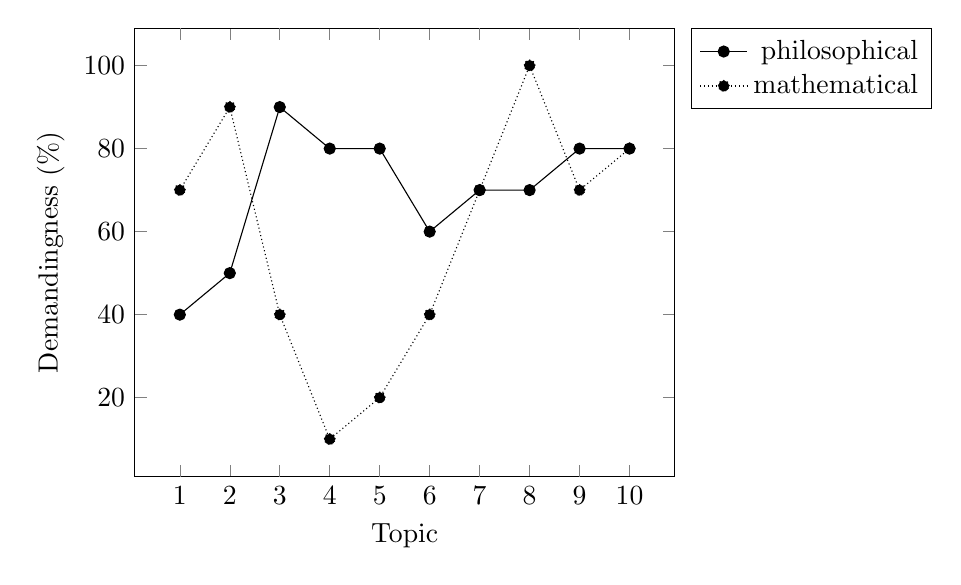
\begin{tikzpicture}
\begin{axis}[
	xlabel={Topic},
	ylabel={Demandingness (\%)},
	extra x ticks={1,3,5,7,9},
	legend style={
		cells={anchor=east},
		legend pos=outer north east,
	},
	cycle list={
		{black,mark=*},
		{densely dotted,mark=*}
	},
]
\addplot coordinates {
	(1,40) (2,50) (3,90) (4,80) (5,80) (6,60) (7,70)  (8, 70) (9, 80) (10, 80)
};

\addplot coordinates {
	(1,70) (2,90) (3,40) (4,10) (5,20) (6,40) (7,70)  (8,100) (9, 70) (10, 80)
};


\legend{philosophical, mathematical}
\end{axis}
\end{tikzpicture}
 
\end{center}


 \begin{itemize}
     \item On the \textbf{philosophical} side, a demandingness level of 100\% means that some of the ideas we'll be discussing are rather subtle; you won't need philosophical training to understand them, but you'll have to think about them very carefully.

\item On the \textbf{mathematical} side, a demandingness level of 100\% means that the material is designed for someone who is familiar with college-level mathematics or is otherwise experienced in mathematical proof.

 \end{itemize}

\vskip.15in
\noindent\textbf{Course Materials:} The primary course materials comprise videos and text on MITx, accessible through Canvas. The most important part is the written text. Focus on that if you want to understand the material (and if you don't want to understand the material, then\dots). You don't need to watch the videos if you don't want to---they have some admittedly awkward camera angles and cuts. They are simply an additional resource for you, including lectures from pre-pandemic times given by Prof. Agust\'{i}n Rayo---the \textit{architect} of this course---along with extras such as interviews with experts. 

% taught the class in previous years and wrote the textbook the class is based on, as well as 

%The MITx materials include videos of three different kinds:

%\begin{itemize}
%    \item  \emph{Lightboard videos:} I use these videos to go over the key concepts of the relevant lecture.  Although they overlap with the written text, I sometimes go about things in a slightly different way, in an effort to give you an alternate perspective.

%\item \emph{Lectures from pre-pandemic times:} These videos often cover similar material to what you'll find in the text, but the material is sometimes presented a bit differently because I gave the lectures several years before I finalized the text.

%\item \emph{Extras:} I posted these videos  in the hope that you might find them interesting or fun. (Sometimes they are interviews with experts in the field; sometimes they are introductions to a topic; sometimes they are animations made to help explain a point.)
%\end{itemize}


In addition to the problem sets posted on Canvas, you'll find exercises scattered throughout the MITx lectures. \textbf{Any answers to these exercises will NOT count toward your grade}. So you shouldn't stress about these exercises, but give `em a try! They'll deepen your understanding of the material, and they are (sometimes) good preparation for problem sets. Like life, some of the exercises are quite tricky. As always, I recommend that you fully and completely accept yourself! 
%But, as I said, don't stress out about them. Instead, 

\vskip.15in
\noindent\textbf{Textbook:} %\footnotemark
There is no required textbook, as all course materials are available on MITx. The MITx materials are based on the book below, which you can buy if you prefer a non-electronic format or if you'd like to retain access to the course materials after the end of the semester. It can be casually read in 20 hours (at roughly a chapter a day, which I'm told keeps ignorance at bay): 

\vspace{1mm}
\begin{center}
  %\includegraphics[width=3.5cm]{cover.png}\\
Rayo, A. \emph{On the Brink of Paradox}, MIT Press, 2019.
\end{center}


\vskip.05in
\noindent\textbf{Lecture:} Hunt will cover the basics in class, introduce additional philosophical content you can't get \textit{anywhere else}, and work through problems with you. We'll be trying out some active learning, which many pedagogical professionals rave about. We'll see if we're left raving or ranting.
%Participation will be assessed in the form of writing a response to a question. Hunt will not painstakingly cover everything, since (i) that would be boring and (ii) we have ample resources to learn the material.  

\vskip.15in
\noindent\textbf{Piazza Wiki:}
The class has a Piazza Wiki, accessible through Canvas. Please use the wiki to ask questions about the class and interact with your fellow students. (\textbf{No answers to problem set questions allowed}!) Posting \textbf{answers} to someone else's questions on Piazza can supplement your participation credit for lecture or recitation, at the generous rate of 0.5 grade-points per substantial answer (up to 2 points total) [perhaps like large cardinals, extra credit does NOT exist in this class].

\vspace*{.15in}
\noindent\textbf{Grading Policy:} 
There will be no final examination. Final grades will be calculated as follows:




\begin{center} \begin{minipage}{6.0in}
\begin{flushleft}
Problem Sets \dotfill 80\% (9 total, lowest score dropped) \\
%Pop Quizzes and Surveys \dotfill 15\% \\
Recitation Participation \dotfill 11\% ($\sim$attend 11 sections \& contribute) \\
Lecture Participation \dotfill 9\% ($\sim$attend 12 lectures \& write something in class) \\
Up to 2 participation grade points can come from answering four Piazza questions \\ 
You can LOSE points if you are rude to a TA or turn in illegible work! (see details below) \\
\end{flushleft}
\end{minipage}
\end{center}

\noindent
\textit{Note well}: Hunt reserves the right to institute in-class quizzes or short philosophical essays if it seems that people are cheating on the problem sets! Odds are high that you won't like this if it comes to it! 

\vspace*{1mm}

\vskip.15in 
\noindent\textbf{Grading Scheme:}

\noindent
Letter Grades as follows: $90 \leq$ A- $<94 \leq$ A $< 98 \leq$ A+ \\
\phantom{Letter Grades as follows:} $80 \leq$ B- $<84 \leq$ B $< 88 \leq$ B+ $< 90$ \\
\phantom{Letter Grades as follows:} $70 \leq$ C- $<74 \leq$ C $< 78 \leq$ C+ $< 80$ \\
\phantom{Letter Grades as follows:} and so on for D range. F $< 60$ (don't do this!). \\[1em] Curving is very unlikely because the class is based largely on problem sets and has participation points!  \\ Modulo concerns about free will in Units 4 \& 5, you control your destiny.  

\iffalse 
\begin{center}\begin{minipage}{3.5in}\begin{multicols}{2}
\begin{flushleft}
\noindent
100\% \dotfill  A+\\
      94--99\% \dotfill A\mbox{\hspace{3mm}}\\
 90--93\% \dotfill A$-$\\
 89\% \dotfill B+\\
 84--88\% \dotfill B\mbox{\hspace{3mm}}\\
 80--83\% \dotfill B$-$\\
  79\% \dotfill C+\\
   74--78\% \dotfill C\mbox{\hspace{3mm}}\\
 70--73\% \dotfill C$-$\\
 60--69\% \dotfill D\mbox{\hspace{3mm}}\\
 0--60\% \dotfill F\mbox{\hspace{3mm}}
\end{flushleft}
\end{multicols}
\end{minipage}\end{center}
\fi 



\vskip.15in
\noindent \textbf{Course Schedule:}
The class comprises 10 non-degenerate modules, each devoted to a topic. \\ The materials for each module will be released sequentially throughout the semester. \\ Almost every module has a problem set. (See the course schedule below for due dates.)

\begin{center}\begin{minipage}{4.5in}
\begin{flushleft}
\item[\textbf{Topic 0: What are we doing here?}]
\item 

\emph{Lecture}: Tuesday, February 7  

\textit{Optional reading}: Maddy (2008) ``How applied math became pure''

\item[\textbf{Topic 1: Infinite Cardinalities}]
\item

\emph{Lecture}: Thursday, February 9

\emph{Recitation}: Friday, February 10 (meet and greet!)
%March 10 is add date 
%April 25 is drop date

\emph{Lecture}: Tuesday, February 14 (Make \textit{math} your Valentine!)

\emph{Lecture}: Thursday, February 16

$\triangleright$ Problem Set 1 due: \textbf{5pm, Sunday, February 19}

\item[\textbf{Topic 2: The Higher Infinite}]
\item 

NO 24.118 on Tuesday, February 21 (follow \textit{Monday} schedule): 

\emph{Lecture}: Thursday, February 23

\emph{Lecture}: Tuesday, February 28

\emph{Lecture}: Thursday, March 2

$\triangleright$ Problem Set 2 due: \textbf{5pm, Sunday, March 5} 

\item[\textbf{Topic 3: Omega-Paradoxes} (ohhmeegaddd)]
\item 

\emph{Lecture}: Tuesday, March 7

\emph{Lecture}: Thursday, March 9

$\triangleright$ PSet 3 due: \textbf{5pm, Sun. March 12} (Spring forward booo!)



\item[\textbf{Topic 4: Time Travel} (we might come back to this)]
\item

\emph{Lecture}: Tuesday, March 14

\emph{Lecture}: Thursday, March 16

$\triangleright$ Problem Set 4 due: \textbf{5pm, Sunday March 19}

\item[\textbf{Topic 5: Newcomb's Problem}]

\item

\emph{Lecture}: Tuesday, March 21

\emph{Lecture}: Thursday, March 23

\emph{Recitation}: Fri., March 24 (\textit{John Wick 4} comes out!!!)

$\triangleright$ Problem Set 5 due: \textbf{5pm, Sunday March 26}

SPRING BREAK: Monday, March 27--Friday, March 31 \\ (do something fun!!! e.g. See \textit{John Wick 4}!)

%\emph{Lecture}: Tuesday, March 28

%$\triangleright$ Problem Set 5 due: \textbf{5pm, Sunday April 3}

\item[\textbf{Topic 6: Probability}]
\item

\emph{Lecture}: Tuesday, April 4

\emph{Lecture}: Thursday, April 6

$\triangleright$ Problem Set 6 due: \textbf{5pm, Sunday April 9}



\item[\textbf{Topic 7: Non-measurable Sets \& Axiom of Choice}]
\item

\emph{Lecture}: Tuesday, April 11

\emph{Lecture}: Thursday, April 13

[N.B.: PSet 7\&8 is a single assignment, due April 23]

%$\triangleright$ Problem Set 7 due: \textbf{5pm, Sunday April 17}

\item[\textbf{Topic 8: Banach--Tarski Theorem (Paradox?)}]

\item

MIT off on Monday, April 17 \#Patriots

\emph{Lecture}: Tuesday, April 18 (have filed your taxes!)

\emph{Lecture}: Thurs., April 20 (Hunt's B-day: so we partayyyyy)

$\triangleright$ Problem Set 7\&8 due: \textbf{5pm, Sunday April 23}

\end{flushleft}\end{minipage}
\end{center}
\pagebreak
\begin{center}\begin{minipage}{4.5 in}
\begin{flushleft}

\item[\textbf{Topic 9: Computability} (bring your calculators!)]
%nominally should do three days on this topic? Agustin did that in 2019 
\item

\emph{Lecture}: Tuesday, April 25

\emph{Lecture}: Thursday, April 27

\emph{Lecture}: Tuesday, May 2

%$\triangleright$ Problem Set 9 due: \textbf{5pm, Sunday, April 30}

$\triangleright$ Problem Set 9 due: \textbf{5pm, Sunday, May 7}

\item[\textbf{Topic 10: Gödel's Incompleteness Theorems}]

\item 

\emph{Lecture}: Thursday, May 4

\emph{Lecture}: Tuesday, May 9
 
\emph{Lecture}: Thursday, May 11
 
$\triangleright$ PSet 10 due: \textbf{5pm, Sun., May 14} (Mother's day!)

\item[\textbf{Topic 11: Philosophy of Math or Thermodynamic Limit!!!}]
 
%\item
 
\emph{Lecture}: Tuesday, May 16


\end{flushleft}\end{minipage}
\end{center}









\vskip.15in
\noindent\textbf{Problem Sets:} Problem sets will be posted on Canvas, and answers must be submitted on Canvas.  
Your submission must be a PDF file (e.g. via a scan of written work). Any pictures, and we'll act like it DIDN'T happen! Show a little professionalism people! 

\begin{itemize}
\item Your TA might have a preference for type-written submissions; they'll let you know. 
\item At any rate, \textbf{Hunt will personally dock 5\% of a PSet assignment} if he learns that a TA is struggling to read your handwriting. If you're unsure whether you're handwriting is easily legible, send a sample to your TA. Different people have different tolerances for this kind of thing, based on their lived experience. (Personally, I get stuck when writing looks like hieroglyphics.)

%Type-written submissions are strongly preferred. Handwritten submissions are only acceptable if: $(i)$ your handwriting is easily legible (as judged by your TA), $(ii)$ you produce a clean version of the document (as opposed to the sheet of paper you used to work out the problems), and $(iii)$ your manuscript has been scanned to high enough standards (as judged by your TA). Note, in particular, that {a garden-variety phone photo won't do}. If you must use your phone for scanning, please make sure you use a scanning app, such as \emph{Adobe Scan}, and make any necessary adjustments to the image before it is uploaded. If you are unsure whether your handwriting or your scanning technology will be up to your TA's standards, make sure you get guidance from them well in advance of the problem set's due date.

\item Your lowest problem set grade will be dropped. If you miss any additional problem sets, however, \textbf{you will not be able to make up for them} (seriously---problems don't grow on trees!). So make sure you don't waste your freebie: keep it in reserve for when you really need it, e.g. toward the end of the semester when your other classes start picking up. 

\item To preserve the energy of our stalwart TAs, we may grade a random subset of the questions 
%on some or all problem-sets, 

\item \textbf{Late assignments will not be accepted}. 

%Even though the class has 10 modules, there will be only 9 problem sets. This is because modules 7 and 8 will have a joint problem set. (The joint problem set isn't worth double: it's worth the same as an ordinary problem set.)

\end{itemize}

\begin{quote}

    

\emph{Collaboration Policy:} It's okay to discuss problem sets with other students who are currently taking the class, but \textbf{you must complete the problem set on your own and provide a list of commentators} by using the ``comment'' box on Canvas when you submit your problem set. If you collaborate, \textbf{failure to submit a list of commentators constitutes plagiarism.}
To make it easy for people to find collaboration partners, I've registered the class on: \url{https://psetpartners.mit.edu}
\iffalse
\begin{center}
\url{https://psetpartners.mit.edu}
\end{center}
\fi 
\vspace{1mm}

\emph{Anonymous Grading:} To mitigate bias, your TA will endeavor to grade each problem set without knowing your identity. To achieve this, we humbly request your help:

\begin{itemize}
    \item Please \underline{do not} include your name on problem set submissions: {include your MIT ID}. 
    
    \item Please \underline{do not} list your collaborators on  problem set submissions. As described above, please list any collaborators using the ``comment'' box on Canvas, as you submit your problem set (or on a separate page at the end of your Pset)
\end{itemize}

\vspace{1mm}

\emph{Policy on Outside Sources:} Consulting published materials is okay. With the exception of course-materials, all sources must be credited, in accordance with MIT's Academic Integrity guidelines. \\
-- Problems or problem sets from previous versions of 24.118 \textbf{DO NOT} count as ``course materials" for present purposes and may not be consulted. Any violation of this policy will be considered plagiarism and will be \textit{aggressively} pursued. \\ -- If you want to curry favor with Hunt, let him know if you come across such contraband! 

\end{quote}

\vskip.15in
\noindent\textbf{Participation Points:}  
You can receive up to 20 participation points over the course of the semester: 11 from attending 11 (out of 13) recitation sections and contributing, 9 from attending 12 lectures (out of 26 total) and writing a response to a philosophical question. Piazza answers can yield 2 points. %No extra credit!
\begin{itemize}
    \item \emph{Attend most recitation sections:} you can earn 0.7 points for attending a recitation and an additional 0.3 points by contributing meaningfully to the discussion (as determined by your TA). Basically, if you're checked-out in class on your laptop or phone, you're not getting those extra 0.3 points! Asking a thoughtful question or offering a thoughtful answer to someone else's question are both good examples of meaningful contributions. \\ -- You can miss two recitations without penalty. 
    
    \item \emph{Attend nearly half the lectures:} you can earn 0.75 points by attending lecture and hand-writing a response to a philosophical question. This question can be asked at any time during the class. If you show up late and miss the question, Hunt may smile gracefully upon you with some pity points. If your answer is radically incomplete or does not seem to be written in good-faith, you will not receive full points. Sorry not sorry! 
    
    %although section attendance is optional,  you can earn up to one participation credit for attending your assigned recitation section from beginning to end and one additional credit for making a meaningful contribution to the discussion. (It is up to your TA to determine what counts as meaningful, but asking a thoughtful question and offering a thoughtful answer to someone else's question are both good examples of meaningful contributions.) Note that you can earn at most two credits per recitation.
    
%    \item \emph{Complete in-class reflections:} the last five minutes of each lecture you will be given prompts that ask you to  will be devoted to  with a five-minute period in which you are asked to reflect on the content covered in the lecture. These reflections might include (i) prompts to formulate questions about the material, (ii) 
    
    \item \emph{Answering questions on Piazza:} you can earn up to two participation points for posting thoughtful answers to someone else's questions on Piazza, with each answer worth half a point. \\ -- Your TA determines what counts as a thoughtful-enough answer. \\ -- A Piazza answer is only eligible for participation credit if it is posted to the entire class.
    
     \item \emph{Don't be rude!:} three ways to win, one way to lose! If Hunt finds out that you have been rude to a TA (either verbally or over email), Hunt will dock 0.5 participation points. Being condescending or demeaning counts as being rude. Your future boss, co-workers, and colleagues will expect you to play nice! Might as well get some practice in. \\ -- You may be rude to Hunt; he can take it (he's also not the one grading your problem sets!)
    
\end{itemize}


%It is your responsibility to inform your TA how you have earned your participation  credits. \textbf{You'll need to input the information on Canvas} in the ``comment'' box when you submit your problem sets, explaining whether, and if so how you have earned participation credits between the submission of this problem set and the previous one (or, for the first problem set, between the submission and the beginning of the semester).  Please keep in mind that misrepresenting your contributions constitutes an infringement of our academic integrity guidelines and can lead to disciplinary action.

%Keep in mind that you can earn no more than two discussion credits per module. A recitation section contribution can only count towards a given module's allotment if it takes place after the course materials for that module have been released and before the module's problem set is due. A Piazza contribution can only count towards a given module's allotment if it is on a topic directly connected to the relevant module and if it is posted at least 24 hours before the module's problem set is due. (When a single contribution might correspond to more than one section, you can choose to use your contribution towards the allotment of any of the relevant modules.)








%for many problems, most of your solutions will look basically identical.  
%What this means: in life, if you're going to cheat, you better trust the people you're cheating with. 

%If you cheat on an exam, there will be hell to pay (i.e. the academic consequences will be severe). But remember: school is just school, and there is much more to life than this. So don't fret about any of this grade stuff. Have fun, be free, and live the life you've imagined. It is more fun to learn and fail than fail to learn. 
%I'm hoping that you don't feel any need to cheat anyways.




\vskip.15in
\noindent\textbf{Exceptions to class policy:} Personal and medical issues can make it hard to focus on academics. If you find that something is getting in the way of your ability to attend class, complete work, or take an exam, you should contact a dean in Student Support Services ($S^{3}$). A dean will provide you with support and work with us to determine next steps. \\ -- We ask that you go to $S^{3}$ so we know you have had a chance to talk through your situation with someone and to connect with any resources you might need. You can reach out to a dean you have worked with in the past, join their virtual help queue (\url{https://sicp-s3.mit.edu/queue}), or e-mail \href{mailto:s3-support@mit.edu}{s3-support@mit.edu}. \\ -- If the $S^3$ dean believes that your situation warrants an exception to standard class policies, please ask them to contact Hunt requesting an exception.

\begin{itemize}
\item See the supplemental ``Health and Wellness Resources'' document for additional resources, \\ therapeutic remarks, and motivational quotes.  
\end{itemize}

%\noindent\textbf{Exceptions to class policy:} If there are exceptional circumstances that prevent you from submitting a problem set on time or earning discussion credits  (e.g.~a medical emergency), your first step should be to contact MIT's Student Support Services ($S^3$). If the $S^3$ Dean believes that your situation warrants an exception to standard class policies, please ask them to contact me requesting the exception. \textbf{I will not consider exceptions unless the request comes from $\bm S^3$}. (I strongly recommend that you contact $S^3$ \emph{before} your assignment is due.)


%\vskip.15in
%\noindent\textbf{Grade Adjustments:} If you feel like you got the wrong grade on an assignment and are not able to sort things out with your TA, you're welcome to send me your assignment for regrading. Please keep in mind, however, that this can cause your grade to go down rather than up. \emph{I am not as tenderhearted as some of my TAs.}

%\vskip.15in
%\noindent\textbf{Zoom Policy:} Office hours and recitation sections will be conducted by Zoom, which will be accessible through Canvas. Zoom sessions will not be recorded, so as to encourage participation. We much prefer it when students keep their video cameras on and are clearly visible on screen, so as to encourage a lively and friendly discussion. But students who would rather keep their camera off will not be penalized or singled out.
 

%\vskip.15in
%\noindent\textbf{Different Time Zones:} I am mindful of the fact that students may be working from different time zones during the pandemic and will do my best to ensure that office hours and recitation section times accommodate as many people as possible. If you are working from a different time zone and feel like you need some sort of accommodation, {please let me know during the first week of class} by taking the welcome survey, which is available through Canvas.




\vskip.15in
\noindent\textbf{Electronic device policy:} if you are gonna use your laptop in class, text your hot date, or otherwise distract yourself, please sit on the RIGHT SIDE of the lecture hall (relative to facing the boards). 

%Laptops, tablets, cellphones and other electronic devices are \emph{not} allowed in class.

\emph{Why?} There is empirical evidence that using electronic devices in class hurts learning---and, in particular, hurts the learning of people around you. So you can all choose to hurt each other's learning! And let people in the left of the hall be spared! LEFT is laptop-free. \#Illiberalism 

%\clearpage 

\vskip.15in
\noindent\textbf{Academic Integrity:}  
\begin{itemize}

\item Any suspicion of plagiarism, cheating, or academic dishonesty will be \textit{aggressively} pursued. \\ You are working with Immanuel Kant in the flesh here, you hear?! Check yo'self before you wreck yo'self: See MIT's Guidelines on Academic Integrity: \url{https://integrity.mit.edu/}.   
 
 \item Blindly copying someone else's solution (either written or typed) counts as cheating. \\ -- In contrast, talking through a solution step-by-step with a classmate---evincing understanding at each step---then writing this solution up yourself step-by-step does NOT count as cheating (even if you end up with nearly identical steps). They see me learnin', they hatin'! 

\end{itemize}

\vskip.05in
\noindent\textbf{Cheating Detection! (buckle up!)}

\begin{itemize}
\item We will avail ourselves of basic game theory: if you gain compelling evidence that a classmate is cheating, you are incentivized to report it to Hunt (and disincentivized to stay quiet). \\ -- Hunt will 100\% honor your confidentiality (ain't no snitchin' from this guy!). 

\item If your report is accurate, you will garner 1\% extra credit (equivalent to 1/10th of a problem-set). The cheater will lose 4\%. Additional correct reports will gain 0.5\% extra credit \\ (up to a maximum of 5\% cheating detection points---One can't pass a class by being a vigilante). 

\item If you gain compelling evidence that someone ELSE knows about cheating but hasn't reported it within 24 hours, you can report that to earn 1\% extra credit (i.e. 1 gradepoint). 
\begin{itemize}
\item The person who failed to report will lose 2\% (i.e. 2 gradepoints). 
\item If all witnesses report, no one loses points except the cheater(s). In this case, no one gains points either (since then you could form cartels to gain extra credit). 
\end{itemize}


\item \textit{What this all means}: if you cheat in a group, you are at the mercy of your group-members. \\ If you witness cheating, but don't report it, you are at the mercy of other witnesses. \\ -- If a cheater reports themselves first, they lose 2\%. (Turn yourself in y'all!)

\item Hunt reserves the right to modify this policy to forestall unethical Nash Equilibria! \\ (e.g. exploiting students in pyramid schemes or enlisting temporary enrollees who later drop). 

\end{itemize}

\vskip.05in
\noindent\textbf{Being for Diversity and Inclusivity:} In all course-related activities and communications, you will be treated with respect. Hunt and the TAs welcome individuals of all ages, backgrounds, beliefs, ethnicities, genders, gender identities, gender expressions, national origins, religious affiliations, sexual orientations, ability, and other visible and non-visible differences. All members of this class are expected to help create a respectful, welcoming, and inclusive environment for every other member of the class who respects this policy. TL;DR: We'll be as inclusive as set theory! 

\vskip.15in
\noindent\textbf{Accommodations:}
Most of us are at best temporarily able-bodied. If you require an accomodation that entails an exception to an aforementioned class policy, please get in touch with Hunt ASAP. For epistemic reasons, Hunt would prefer if you have some record or note from Disability and Access Services at \href{mailto:das-student@mit.edu}{das-student@mit.edu} (or for assistive technology, \href{mailto:atic-staff@mit.edu}{atic-staff@mit.edu}), but he understands from personal experience that sometimes these are hard to come by in a timely manner (American medical system blah blah Joe Biden's America blah blah). 




%If you are a student with learning needs that require special accommodation, contact Disability and Access Services at das-student@mit.edu (or for assistive technology, atic-staff@mit.edu) as soon as possible, to make an appointment to discuss your needs and to obtain an accommodations letter.  Please e-mail me as soon as possible to set up a time to discuss your learning needs. As someone who has used these services in the past, you can assume that I will be HIGHLY sympathetic!

%Students with disabilities are welcome in this class. If you require an exception to class policies because of a disability, please contact Student Disability Services and ask them to send me a request on your behalf. 



















%%%%%% END 
\end{document} 